\documentclass{article}

\usepackage[hscale=0.8,vscale=0.8]{geometry}
\usepackage{graphicx}
\usepackage{listings}
\graphicspath{ {./} }

\pagenumbering{gobble}

\begin{document}

\title{Project 2 Answers}	

\paragraph*{Approach \& Steps}
\paragraph{I started with trying to make a simple mesh as mentioned by professor. The first mesh was cylindrical in nature and had a lot of spaces left out on the top right corner, where the elements were very coarse. Then, I used the cylindrical coordinate approach, where I used sin, cos and tan to make a uniform regular mesh. Once I had the mesh, I wrote the code for performing FEA, which was straight forward. I got the results for displacement. Further, I wrote the code for calculating the stress at point C. Here, I faced a critical issue. In the uniform mesh, the elements near the elliptical region remained uniform to the ones on the edges. The $\sigma_y$ drops exponentially as we move away from Point 'C'. This led to inaccurate results in the solution. The Solution was moving towards the Inglis Analytical results, but, needed huge computational Power to do so. Furthermore, This led me to developing a non-uniform mesh that could help me implement finer meshing near the ellipse and let the meshing at the far end of the plate uniform. Thus, I finally implement the non-uniform mesh with a mesh gradient.}

\paragraph{The idea was to increase the distance between any two consecutive nodes by a factor of the gradient, thus giving us a geometric series. Let's say the x is the total length to be meshed. Then, we keep the first point as $ k*x $, and each consecutive distance is $ k*x^i$ , till $i = n-1 $. Furthermore, adding up all the distances, we get the value of k, implemented in the Final code.}

\paragraph*{Comparison with Theoretical Solution}

\paragraph{The \underline{Inglis} solution provides the value of $ 6 * 10^8 $ and the solution I get for the chosen parameters is $ 5.98 * 10 ^ 8 $. The Solution matches closely as due to the non-uniform meshing, we have a denser mesh near the elliptical region, giving more accuracy alongside a reasonably accurate solution for areas with comparatively less dense mesh. Furthermore, as can be seen in the first plot, The Inglis solution is not matching accurately at the start and matches closely at the end. This also implies high amount of stress localization at point C when the value of b is 0.001.}

\paragraph*{Design Recommendations}

\paragraph{It can be clearly seen that as the value of the minor Axis b decreases, the Amount of maximum stress increases exponentially. That is an important factor to consider during designing a plate with hole. Furthermore, it also shows that the cracks have a lot more stress in it and tend to fracture. Thus, this accounts for important observation to be considered during the study related to fracture Mechanics of plate. My Design would try to incorporate stress loading such that there is a trade off of displacement and stress. I would try to keep my stress as minimal as possible, given my displacements are still within the tolerance specified/decided.}

\begin{figure}[t]
	part 9 : Design Recommendations
	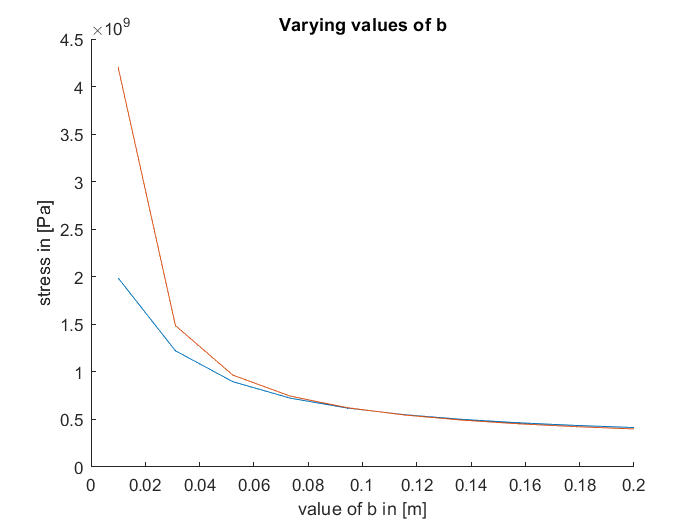
\includegraphics[width=20cm]{tot_ingle_comp}
	\centering
\end{figure}


\paragraph{All the Plots and Contours have been added below. The Code(Converted to PDF) and the Table for Coordinates is attached at the end of this PDF.}


\begin{figure}[t]
	ii : Convergence Study
	\includegraphics[width=20cm]{convergence study}
	\centering
\end{figure}

\begin{figure}[t]
	v : Deformed \& Un Deformed Mesh
	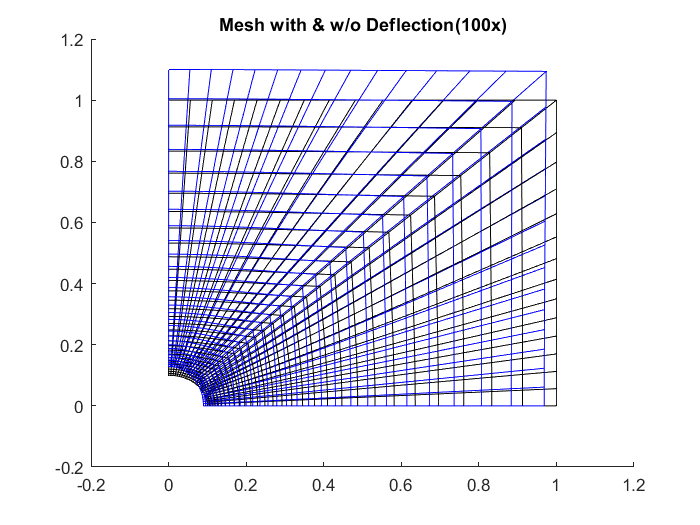
\includegraphics[width=20cm]{mesh}
	\centering
\end{figure}

\begin{figure}[t]
	vi : Von Misses Stress in Plate
	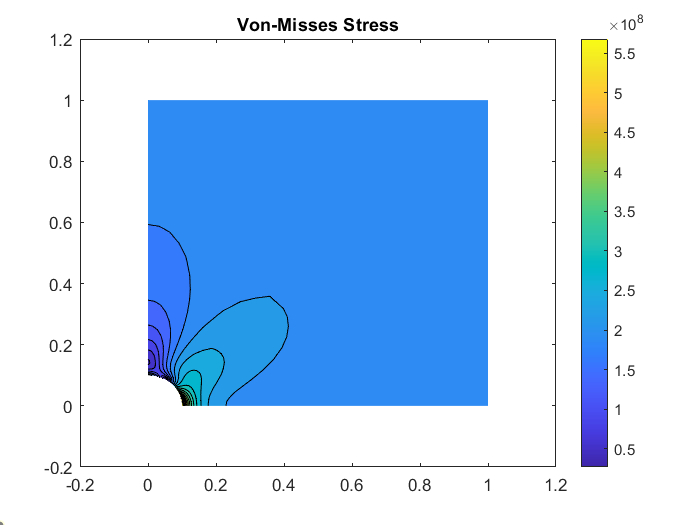
\includegraphics[width=20cm]{vm_stress}
	\centering
\end{figure}

\begin{figure}[t]
	vii : Principal Stress in Y direction
	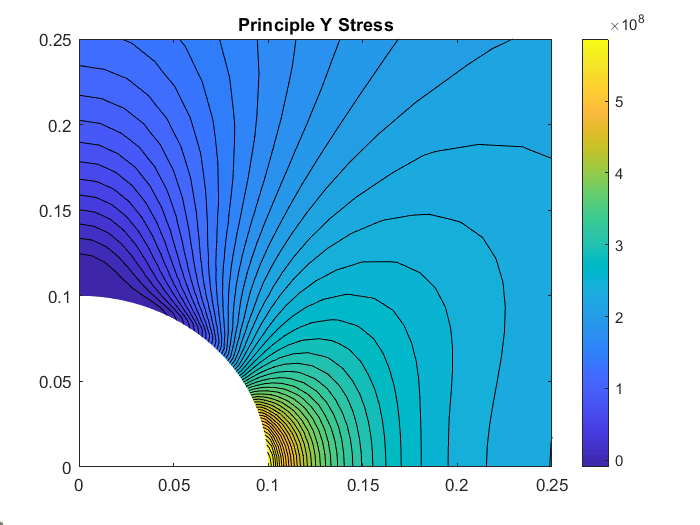
\includegraphics[width=20cm]{principal_near}
	\centering
\end{figure}

\begin{figure}[t]
	viii : Principal Stress in Y direction for b = 0.01
	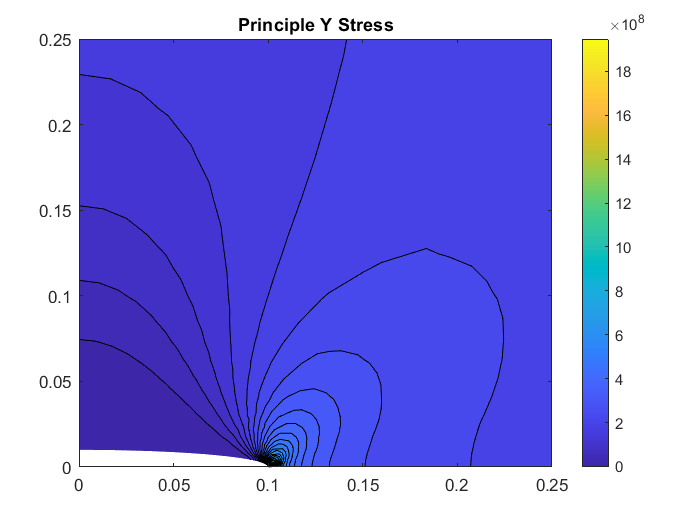
\includegraphics[width=20cm]{principal_near_max}
	\centering
\end{figure}
	
\end{document}